\title{Conforming Voronoi Meshing Based on Maximal Poisson Sampling}
\author{} \institute{}
\tocauthor{\underline{M.~S.~Ebeida}, P.~Knupp, V.~Leung}
\maketitle

\begin{center}
{\large \underline{Mohamed Ebeida}, Patrick Knupp, Vitus Leung}\\
Sandia National Laboratories\\
{\tt msebeid@sandia.gov, pknupp@sandia.gov, vleung@sandia.gov}
\end{center}

\section*{Abstract}
We present a conforming Voronoi meshing algorithm for non-convex domains with internal features. Based on a uniform distance function, our algorithms starts with generating a bias-free random point cloud within the domain boundaries. This bias-free feature is crucial for simulations of propagating cracks since it minimizes the effect of the tessellation on the direction of the crack growth. The generated point cloud satisfies the requirements of maximal Poisson sampling, leading to a constrained Voronoi mesh with guaranteed angle bounds. The presented algorithm is linear in the number of generated points and can be efficiently implemented in parallel. Several examples are presented below to show the capabilities of this new approach.

\begin{figure}[htb]
\centering
{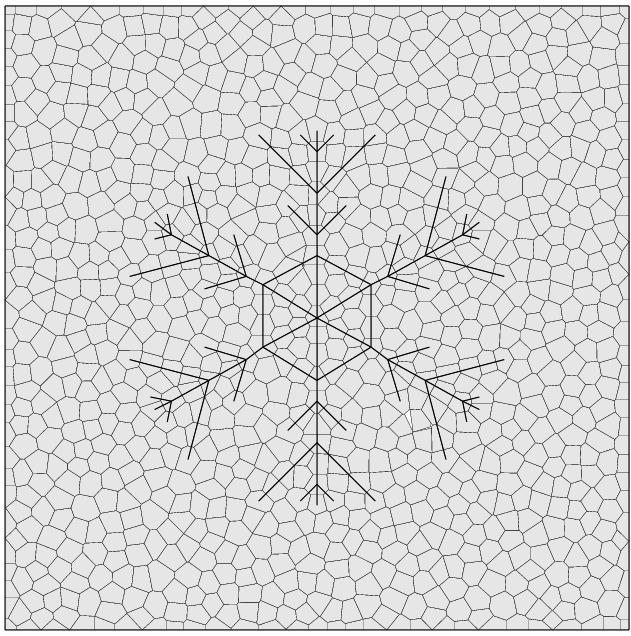
\includegraphics[height=3.7cm]{./ebeida/snowflake_voronoi.png}}$\,$
{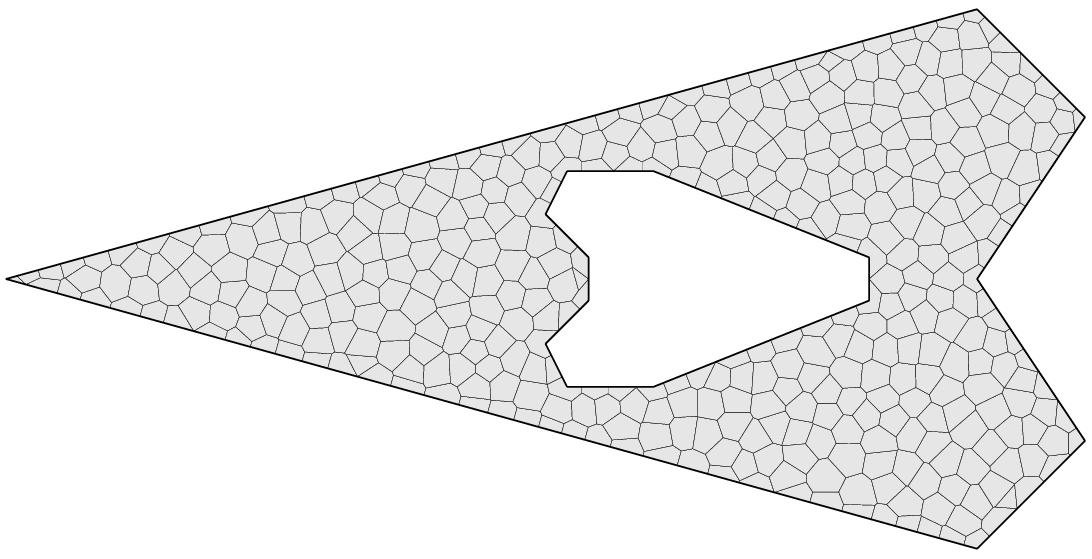
\includegraphics[height=3.7cm]{./ebeida/wedge_voronoi.png}} $\,$
{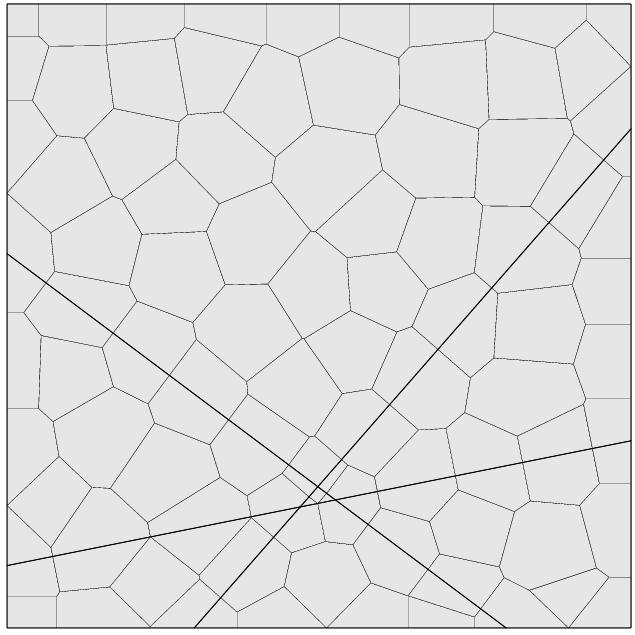
\includegraphics[height=3.7cm]{./ebeida/cracks_voronoi.png}}
\caption{Conforming Voronoi Tessellations based on a uniform distance function for a square domain with internal boundaries (left), a non-convex domain with a hole (middle) and a square domain with multiple regions in contact (right). A serial implementation of our algorithm is capable of distributing 100,000 random points/second and tessellating the output point cloud at a rate of 250,000 points/second}
\label{fig:cdt_steps}
\end{figure}